\documentclass[10pt,twocolumn]{article}


\usepackage{two-row-acad-cv}


\colorlet{cvthemecolour}{black}
%------------------------------------------------------------
% put in another colour instead of cyan to change the colour
%------------------------------------------------------------
\colorlet{cvcolour}{cyan}


\begin{document}

% -----------------------------------------------------------
% the NAME
% -----------------------------------------------------------
\nametag{Pascal P. }{Klamser}
\headerrule{cvcolour}{0.6cm}

% -----------------------------------------------------------
% The PHOTO and INFO BOX
% -----------------------------------------------------------
\fbox{
\begin{minipage}[t]{0.20\textwidth}
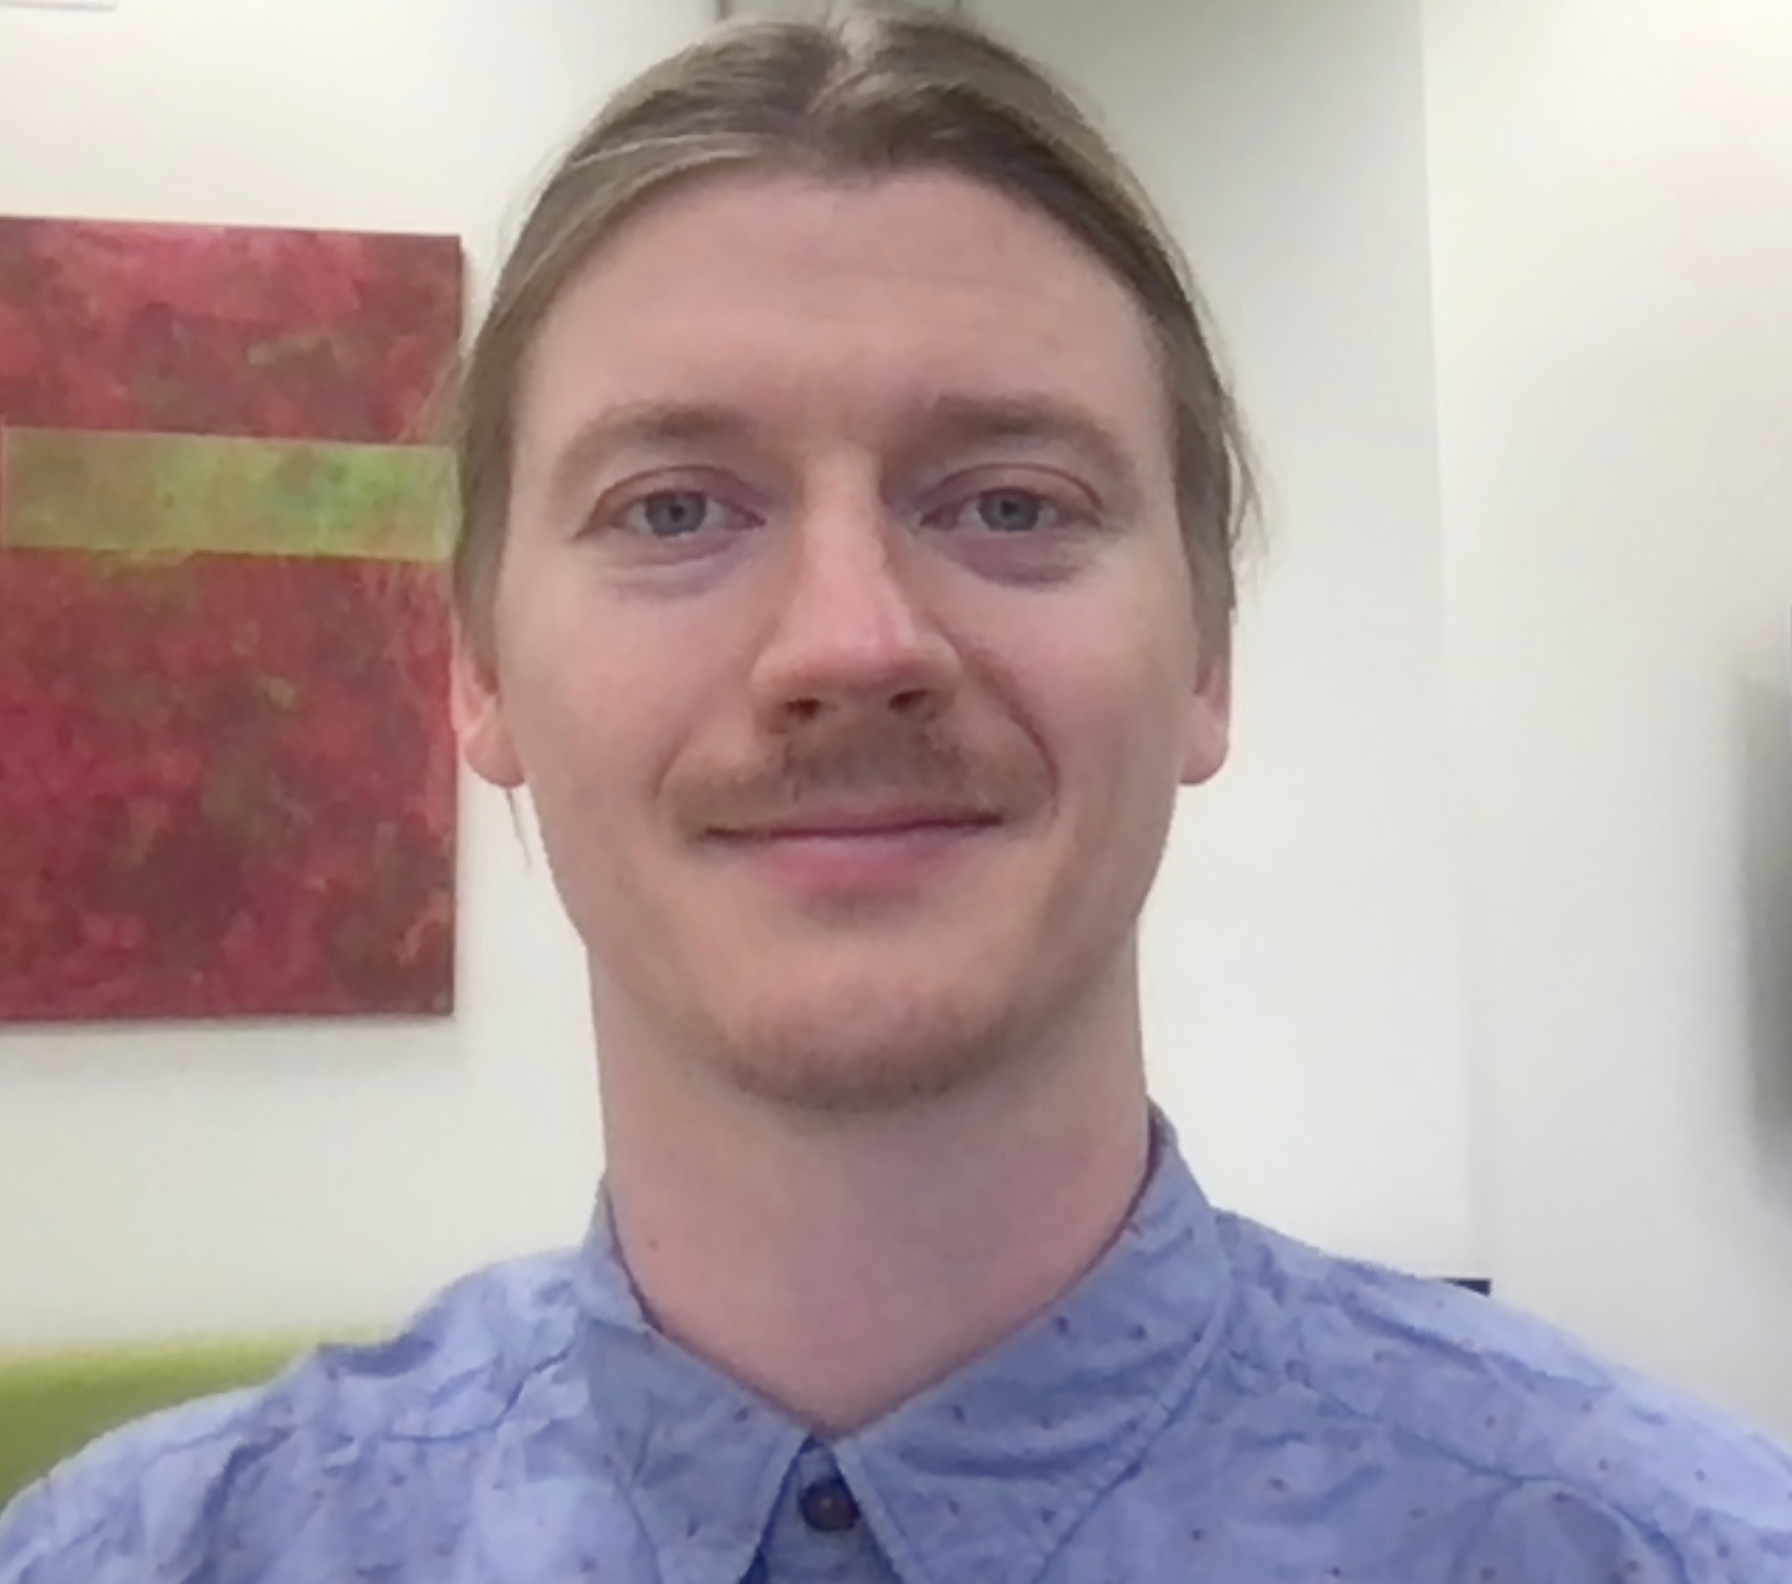
\includegraphics[valign=t,width=\textwidth]{pascal_color.png}
\end{minipage}% \hspace{1em}\hfill
\begin{minipage}[t]{0.24\textwidth}
\vspace{1em}


\begin{tabular}{r|>{\footnotesize}p{0.65\textwidth}}
    \faPhone & +49/xxxxxxxxxxx \\
    \faHome & xxxxxxxxxxxx \\
    \faMapMarker & Berlin, Germany \\
    \faAt & \href{mailto:klamser@physik.hu-berlin.de}{click to mail me} \\
    \faLaptop & \href{https://github.com/PaPeK}{github.com/PaPeK}
\end{tabular}
% \vspace{1em}
\end{minipage}
}
% -----------------------------------------------------------

\vspace{2em}

\begin{sansserif}
Pascal P. \kursiv{Klamser} is an interdisciplinary scientist.
He started as physicist with a focus in statistical physics and dynamical systems.
During his MSc he studied bifurcation predictions and opinion dynamics \cite{klamser_zealotry_2017}.
His PhD in biophysics focused on collective information processing and criticality
in animal groups \cite{klamser_collective_2021, klamser_impact_2021, lukas_acoustic_2021, lukas_diurnal_2021, sbragaglia_evolutionary_2022, doran_fish_2022, gomez-nava_fish_2023}.
During his PostDoc and COVID-19, he processed daily mobility and contact data and
communicated it to health officials and the public \cite{maier_germanys_2022, maier_estimating_2023}. 
His current interests are fungal growth networks,
the worldwide aviation network\cite{klamser_enhancing_2023, klamser_inferring_2024} and fish track behavioral classification.


\end{sansserif}

\cvrule{black}{2pt}


\subsection{Education}
\begin{tabular}{r|l r}
    2021 & PhD Biophysics, \textit{HU Berlin} &magna c. l.\\
    2016 & MSc. Physics, \textit{HU Berlin} &1.4\\
    2014 & Erasmus, \textit{EPFL} Switzerland & \\
    2013 & BSc. Physics, \textit{HU Berlin} &2.5\\
    2007 & Abitur, \textit{Gymnasium Egeln} &1.7 
\end{tabular}

\cvrule{black}{2pt}

\subsection{Theses}
{\renewcommand{\arraystretch}{1.4}
\begin{tabular}{r|p{0.4\textwidth}}
    PhD &  Collective Infromation Processing and Criticality, Evolution and Limited Attention {\footnotesize (supervision: Prof. Pawel Romanczuk)}\\
    MSc &  Multidimensional Optimization of Bifurcation Predictions {\footnotesize (supervision: Prof. Jürgen Kurths)}\\
    BSc &  {\footnotesize Installation of a Magneto- Optic Kerr Effect Setup to Investigate the Effect of a Ta Buffer Layer on the Magnetic Properties of a Co/FeMn Bilayer System (supervision: Dr. Florian Kronast)}
\end{tabular}
}


\cvrule{black}{2pt}


\subsection{WORK EXPERIENCE}
\begin{tabular}{p{0.05\textwidth}| p{0.35\textwidth}}
    \cvevent{2024}{Post Doc}
        {\href{https://synosys.github.io/}{SynoSys @ tud} \color{cvcolour}}
        {Dresden}
        {Modeling of fungal growth networks~\textbf{|}
        Mobility analysis of the aviation data~\textbf{|}
        MySQL and PostgreSQL server admin}
        {Python, MySQL, PostgreSQL}\\
    \cvevent{2023--2024}{Data Scientist}
        {\href{https://www.rki.de/DE/Content/Institut/OrgEinheiten/ZIG/ZIG-WHO-HUB/ZIG_WHO_HUB_node.html}{zig rki who hub}}
        {Berlin}
        {Text analysis of \href{https://www.who.int/initiatives/eios}{EIOS data}~\textbf{|}
        Noise reduction in search queries~\textbf{|}
        Posit server setup and admin}
        {Python, Elasticsearch, BERT, Posit}\\
    \cvevent{2021--2023}{Post Doc}
        {\href{https://synosys.github.io/}{brockmann lab @ rki} \color{cvcolour}}
        {Berlin}
        {German mobility and contact data analysis and visualization~\textbf{|}
        Epidemic modelling incorporating aviation data~\textbf{|}
        Teamlead in the \href{https://www.covid-19-mobility.org/}{Covid-19 Mobility Project}}
        {Python, MySQL, R, Hugo}\\
    \cvevent{2016--2021}{PhD Student}
        {\href{http://lab.romanczuk.de/}{romanczuk lab} \color{cvcolour}}
        {Berlin}
        {Agent based modelling of collective behavior with~\textbf{|}
        Data analysis of animal tracks~\textbf{|}
        Application of CNN for animal detection }
        {C++, Python, Processing, Keras, pytorch}
\end{tabular}

\cvrule{black}{2pt}

\renewcommand\bibname{Publications}
\renewcommand{\refname}{Publications}

\begin{thebibliography}{10}

\bibitem{klamser_zealotry_2017}
\textbf{Pascal~P. Klamser}, Marc Wiedermann, Jonathan~F. Donges, and Reik~V. Donner.
\newblock Zealotry effects on opinion dynamics in the adaptive voter model.
\newblock {\em Physical Review E}, 96(5):052315, 2017.

\bibitem{klamser_collective_2021}
\textbf{Pascal~P. Klamser} and Pawel Romanczuk.
\newblock Collective predator evasion: Putting the criticality hypothesis to the test.
\newblock {\em {PLOS} Computational Biology}, 17(3):e1008832, 2021.

\bibitem{klamser_impact_2021}
\textbf{Pascal~P. Klamser}, Luis Gómez-Nava, Tim Landgraf, Jolle~W. Jolles, David Bierbach, and Pawel Romanczuk.
\newblock Impact of variable speed on collective movement of animal groups.
\newblock {\em Frontiers in Physics}, 9:715996, 2021.
\newblock \textbf{shared first authorship}.

\bibitem{lukas_acoustic_2021}
Juliane Lukas, Pawel Romanczuk, Haider Klenz, \textbf{Pascal~P. Klamser}, Lenin Arias~Rodriguez, Jens Krause, and David Bierbach.
\newblock Acoustic and visual stimuli combined promote stronger responses to aerial predation in fish.
\newblock {\em Behavioral Ecology}, 32(6):1094--1102, 2021.

\bibitem{lukas_diurnal_2021}
Juliane Lukas, Felix Auer, Tobias Goldhammer, Jens Krause, Pawel Romanczuk, \textbf{Pascal~P. Klamser}, Lenin Arias-Rodriguez, and David Bierbach.
\newblock Diurnal changes in hypoxia shape predator-prey interaction in a bird-fish system.
\newblock {\em Frontiers in Ecology and Evolution}, 9:619193, 2021.

\bibitem{sbragaglia_evolutionary_2022}
Valerio Sbragaglia, \textbf{Pascal~P. Klamser}, Pawel Romanczuk, and Robert Arlinghaus.
\newblock Evolutionary impact of size-selective harvesting on shoaling behavior: Individual-level mechanisms and possible consequences for natural and fishing mortality.
\newblock {\em The American Naturalist}, 199(4):480--495, 2022.
\newblock \textbf{shared first authorship}.

\bibitem{doran_fish_2022}
Carolina Doran, David Bierbach, Juliane Lukas, \textbf{Pascal~P. Klamser}, Tim Landgraf, Haider Klenz, Marie Habedank, Lenin Arias-Rodriguez, Stefan Krause, Pawel Romanczuk, and Jens Krause.
\newblock Fish waves as emergent collective antipredator behavior.
\newblock {\em Current Biology}, 32(3):708--714.e4, 2022.

\bibitem{gomez-nava_fish_2023}
Luis Gómez-Nava, Robert~T. Lange, \textbf{Pascal~P. Klamser}, Juliane Lukas, Lenin Arias-Rodriguez, David Bierbach, Jens Krause, Henning Sprekeler, and Pawel Romanczuk.
\newblock Fish shoals resemble a stochastic excitable system driven by environmental perturbations.
\newblock {\em Nature Physics}, 19(5):663--669, 2023.

\bibitem{maier_germanys_2022}
Benjamin~F. Maier, Marc Wiedermann, Angelique Burdinski, \textbf{Pascal~P. Klamser}, Mirjam~A. Jenny, Cornelia Betsch, and Dirk Brockmann.
\newblock Germany’s fourth {COVID}-19 wave was mainly driven by the unvaccinated.
\newblock {\em Communications Medicine}, 2(1):116, 2022.

\bibitem{maier_estimating_2023}
Benjamin~F. Maier, Annika~H. Rose, Angelique Burdinski, \textbf{Pascal~P. Klamser}, Hannelore Neuhauser, Ole Wichmann, Lars Schaade, Lothar~H. Wieler, and Dirk Brockmann.
\newblock Estimating the share of {SARS}-{CoV}-2-immunologically naïve individuals in germany up to june 2022.
\newblock {\em Epidemiology and Infection}, 151:e38, 2023.

\bibitem{klamser_enhancing_2023}
\textbf{Pascal~P. Klamser}, Valeria d’Andrea, Francesco Di~Lauro, Adrian Zachariae, Sebastiano Bontorin, Antonello Di~Nardo, Matthew Hall, Benjamin~F Maier, Luca Ferretti, Dirk Brockmann, and Manlio De~Domenico.
\newblock Enhancing global preparedness during an ongoing pandemic from partial and noisy data.
\newblock {\em {PNAS} Nexus}, 2(6):pgad192, 2023.
\newblock \textbf{shared first authorship}.

\bibitem{klamser_inferring_2024}
\textbf{Pascal~P. Klamser}, Adrian Zachariae, Benjamin~F. Maier, Olga Baranov, Clara Jongen, Frank Schlosser, and Dirk Brockmann.
\newblock Inferring country-specific import risk of diseases from the world air transportation network.
\newblock {\em {PLOS} Computational Biology}, 20(1):e1011775, 2024.

\end{thebibliography}

% 
% \subsection{Teaching Experience}
% \begin{tabular}{r| p{0.7\textwidth}}
%     \cvevent{2018--2021}{Captain of the Black Pearl}{Lead}{East Indies \color{cvcolour}}{Finally got the goddamn ship back.}{disney.png} \\
%     \cvevent{2019}{Freelance Pirate}{Bucaneering}{Tortuga \color{cvcolour}}{This and that. The usual, aye?}{medal.jpeg} \\
%     \cvevent{2016--2017}{Captain of the Black Pearl}{Lead}{Tortuga \color{cvcolour}}{Found a secret treasure, lost the ship.}{medal.jpeg}
% \end{tabular}
% 
% 
% \vspace{5em}
% 
% \section{TEACHING STATEMENT}
% \lipsum[23]
% 
% \cvrule{black}{2pt}

% to change References --> Publications
\bibliographystyle{unsrt}
% \bibliography{PsPaper}




\end{document}